\documentclass{article}
\usepackage{physics}
\usepackage{graphicx}
\usepackage{caption}
\usepackage{amsmath}
\usepackage{bm}
\usepackage{framed}
\usepackage{authblk}
\usepackage{empheq}
\usepackage{amsfonts}
\usepackage{esint}
\usepackage[makeroom]{cancel}
\usepackage{dsfont}
\usepackage{centernot}
\usepackage{mathtools}
\usepackage{bigints}
\usepackage{amsthm}
\theoremstyle{definition}
\newtheorem{defn}{Definition}[section]
\newtheorem{prop}{Proposition}[section]
\newtheorem{rmk}{Remark}[section]
\newtheorem{thm}{Theorem}[section]
\newtheorem{exmp}{Example}[section]
\newtheorem{prob}{Problem}[section]
\newtheorem{sln}{Solution}[section]
\newtheorem*{prob*}{Problem}
\newtheorem{exer}{Exercise}[section]
\newtheorem*{exer*}{Exercise}
\newtheorem*{sln*}{Solution}
\usepackage{empheq}
\usepackage{tensor}
\usepackage{xcolor}
%\definecolor{colby}{rgb}{0.0, 0.0, 0.5}
\definecolor{MIT}{RGB}{163, 31, 52}
\usepackage[pdftex]{hyperref}
%\hypersetup{colorlinks,urlcolor=colby}
\hypersetup{colorlinks,linkcolor={MIT},citecolor={MIT},urlcolor={MIT}}  
\usepackage[left=1in,right=1in,top=1in,bottom=1in]{geometry}

\usepackage{newpxtext,newpxmath}
\newcommand*\widefbox[1]{\fbox{\hspace{2em}#1\hspace{2em}}}

\newcommand{\p}{\partial}
\newcommand{\R}{\mathbb{R}}
\newcommand{\C}{\mathbb{C}}
\newcommand{\lag}{\mathcal{L}}
\newcommand{\nn}{\nonumber}
\newcommand{\ham}{\mathcal{H}}
\newcommand{\M}{\mathcal{M}}
\newcommand{\I}{\mathcal{I}}
\newcommand{\K}{\mathcal{K}}
\newcommand{\F}{\mathcal{F}}
\newcommand{\w}{\omega}
\newcommand{\lam}{\lambda}
\newcommand{\al}{\alpha}
\newcommand{\be}{\beta}
\newcommand{\x}{\xi}

\newcommand{\G}{\mathcal{G}}

\newcommand{\f}[2]{\frac{#1}{#2}}

\newcommand{\ift}{\infty}

\newcommand{\lp}{\left(}
\newcommand{\rp}{\right)}

\newcommand{\lb}{\left[}
\newcommand{\rb}{\right]}

\newcommand{\lc}{\left\{}
\newcommand{\rc}{\right\}}


\newcommand{\V}{\mathbf{V}}
\newcommand{\U}{\mathcal{U}}
\newcommand{\Id}{\mathcal{I}}
\newcommand{\D}{\mathcal{D}}
\newcommand{\Z}{\mathcal{Z}}

%\setcounter{chapter}{-1}


\usepackage{enumitem}



\usepackage{subfig}
\usepackage{listings}
\captionsetup[lstlisting]{margin=0cm,format=hang,font=small,format=plain,labelfont={bf,up},textfont={it}}
\renewcommand*{\lstlistingname}{Code \textcolor{violet}{\textsl{Mathematica}}}
\definecolor{gris245}{RGB}{245,245,245}
\definecolor{olive}{RGB}{50,140,50}
\definecolor{brun}{RGB}{175,100,80}

%\hypersetup{colorlinks,urlcolor=colby}
\lstset{
	tabsize=4,
	frame=single,
	language=mathematica,
	basicstyle=\scriptsize\ttfamily,
	keywordstyle=\color{black},
	backgroundcolor=\color{gris245},
	commentstyle=\color{gray},
	showstringspaces=false,
	emph={
		r1,
		r2,
		epsilon,epsilon_,
		Newton,Newton_
	},emphstyle={\color{olive}},
	emph={[2]
		L,
		CouleurCourbe,
		PotentielEffectif,
		IdCourbe,
		Courbe
	},emphstyle={[2]\color{blue}},
	emph={[3]r,r_,n,n_},emphstyle={[3]\color{magenta}}
}






\begin{document}
	
\begin{framed}
	\noindent Name: \textbf{Huan Q. Bui}\\
	Course: \textbf{8.309 - Classical Mechanics III}\\
	Problem set: \textbf{\#7}
\end{framed}



\noindent \textbf{1. Perturbation Theory for Two Springs}

\begin{enumerate}[label=(\alph*)]
	\item The best way to get the Hamiltonian is perhaps through the Lagrangian. The Lagrangian for this system is 
	\begin{align*}
	\lag = \f{1}{2}m \dot{x}^2 - k\lp a\sqrt{1 + \sin^2\theta}- b \rp ^2
	\end{align*}
	where we don't have the factor of $1/2$ in front of $k$ because there are two springs. Since $x = a\sin\theta$ we have
	\begin{align*}
	\lag = \f{1}{2}m a^2\cos^2\theta\dot\theta^2 - k\lp a\sqrt{1 + \sin^2\theta} - b\rp ^2
	\end{align*}
	By definition, 
	\begin{align*}
	p_\theta = \f{\p \lag}{\p \dot{\theta}} = ma^2\cos^2\theta \dot\theta.
	\end{align*}
	With this, we can find $\dot\theta$ in terms of $p_\theta$. Once this is done, we can plug back into the Lagrangian and get the Hamiltonian as follows:
	\begin{align*}
	\boxed{\ham = \f{p_\theta^2}{2ma^2 \cos^2\theta} + k\lp a\sqrt{1+\sin^2\theta} -b \rp^2}
	\end{align*}
	
	Mathematica code:
	\begin{lstlisting}
	In[17]:= L = (1/2)*m*vx^2 - k*(b + a*Sqrt[1 + Sin[\[Theta][t]]^2])^2
	
	Out[17]= -k (b + a Sqrt[1 + Sin[\[Theta][t]]^2])^2 + 
	1/2 a^2 m Cos[\[Theta][t]]^2 Derivative[1][\[Theta]][t]^2
	
	In[18]:= vx = D[a*Sin[\[Theta][t]], t];
	
	In[10]:= (*Velocities in terms of momenta*)
	
	In[19]:= D[L, \[Theta]'[t]]
	
	Out[19]= a^2 m Cos[\[Theta][t]]^2 Derivative[1][\[Theta]][t]
	
	In[20]:= velocities = 
	Solve[{p\[Theta][t] == D[L, \[Theta]'[t]]}, {\[Theta]'[t]}][[1]];
	
	In[8]:= (*Hamiltonian*)
	
	In[21]:= H = p\[Theta][t]*\[Theta]'[t] - L /. velocities
	
	Out[21]= (p\[Theta][t]^2 Sec[\[Theta][t]]^2)/(2 a^2 m) + 
	k (b + a Sqrt[1 + Sin[\[Theta][t]]^2])^2
	\end{lstlisting}
	
	\item The expansion of $1/\cos^2(\theta)$ around $\theta = 0$ reads
	\begin{align*}
	\f{1}{\cos^2\theta} \approx 1 + \theta^2 + \f{2\theta^4}{3} + \dots 
	\end{align*} 
	Thus, the approximate Hamiltonian is 
	\begin{align*}
	\ham &\approx \f{p_\theta^2}{2ma^2}\lp 1 + \theta^2 + \f{2\theta^4}{3} + \dots  \rp \\
	&\quad+ k(a-b)^2 + ka(a-b)\theta^2 + \f{1}{12}ka(7b -4a)\theta^4  + \dots
	\end{align*}
	
	
	The constant does not change the dynamics of the system, so we may ignore it. We thus identify 
	\begin{align*}
	\ham_0 
	&= \f{p_\theta^2}{2ma^2} + ka(a-b)\theta^2 \\
	&= \f{1}{2ma^2}\lb p_\theta^2 + (ma^2)^2 \f{2ka(a-b)}{ma^2}\theta^2  \rb\\
	&= \f{1}{2ma^2}\lb p_\theta^2 + (ma^2)^2 \f{2k(a-b)}{ma}\theta^2  \rb\\
	&= \boxed{\f{1}{2I}\lp p_\theta^2 + I^2 \Omega^2 \theta^2 \rp}
	\end{align*}
	has the form of the usual harmonic oscillator. Here we have defined the ``monentum of inertia'' $I = ma^2$ and frequency $\Omega^2 = 2k(a-b)/ma$. The first order correction for this Hamiltonian is 
	\begin{align*}
	\boxed{\Delta \ham = \f{p_\theta^2\theta^2}{2ma^2} + \f{ka}{12}(7b - 4a) \theta^4}
	\end{align*}
	
	Mathematica code:
	\begin{lstlisting}
	(*Expansion of potential in theta*)
	
	In[22]:= k*
	Series[(a*Sqrt[1 + Sin[\[Theta]]^2] - b)^2, {\[Theta], 0, 6}]
	
	Out[22]= SeriesData[\[Theta], 0, {(a - b)^2 k, 0, a (a - b) k, 
	0, (Rational[1, 4] a^2 + Rational[-7, 12] a (a - b)) k, 
	0, (Rational[-7, 24] a^2 + Rational[121, 360] a (a - b)) k}, 0, 7,
	1]
	
	In[26]:= (*Expand 1/cos^2*)
	
	In[28]:= Series[Sec[x]^2, {x, 0, 4}]
	
	Out[28]= SeriesData[x, 0, {1, 0, 1, 0, 
	Rational[2, 3]}, 0, 5, 1]
	\end{lstlisting}
	
	
	\item From $\ham_0$ we find a suitable set of canonical variables corresponding to a vanishing $K$ for the unperturbed system as the usual action variable $J$ and the phase angle $\be$ in the angle variable $w$:
	\begin{align*}
	\al = \ham_0 = \f{\Omega}{2\pi} J \quad\text{and}\quad
	w = \f{\Omega}{2\pi} t + \be
	\end{align*}
	We now solve for $\theta, p_\theta$ in terms of these variables:
	\begin{align*}
	&\theta = \sqrt{\f{2\al}{I \Omega^2 }} \sin(\Omega t + \delta) = \sqrt{\f{J}{\pi I \Omega}} \sin[2\pi(\nu t + \be)]\\
	&p_\theta = \sqrt{2\al I }\cos(\Omega t + \delta) = \sqrt{\f{I J \Omega}{\pi}}\cos[2\pi(\nu t + \be)]
	\end{align*}
	where $\nu = \Omega/2\pi$. Since $\be$ and $w$ are linearly related, the pair $(J,\be)$ is canonical. We can thus use $(J,\be)$ as new canonical variables. Let $J_0$ and $\be_0$ be constants fixed by initial conditions. Then in terms of the new variables, $\Delta \ham$ is 
	\begin{align*}
	\Delta \ham 
	&= \f{p_\theta^2\theta^2}{2ma^2} + \f{ka}{12}(7b - 4a) \theta^4 \\
	&= \f{J^2}{2ma^2\pi^2} \cos^2[2\pi(\nu t + \be)] \sin^2[2\pi(\nu t + \be)] + \f{(7b-4a)J^2}{24a^2(a-b)m\pi^2}   \sin^4[2\pi(\nu t + \be)].
	\end{align*}
	Next we compute the first order corrections to these new variables:
	\begin{align*}
	\dot\be^{(1)} &= \f{\p \Delta \ham}{\p J}\bigg\vert_0 \\
	&=  \frac{J_0  }{24 \pi ^2 a^2 m (a-b)} [(16 a-19 b) \cos [4 \pi  (\beta_0 +\nu  t)] + 8 a-5
	b] \sin ^2[2 \pi  (\beta_0 +\nu  t)] 
	\end{align*}
	and 
	\begin{align*}
	\dot J^{(1)}&= -\f{\p \Delta \ham}{\p \be}\bigg\vert_0  \\
	&=\frac{J_0^2  }{12 \pi  a^2 m (a-b)} [(19 b-16 a) \cos [4 \pi  (\beta_0 +\nu  t)]+4 a-7
	b] \sin [4 \pi  (\beta_0 +\nu  t)]
	\end{align*}
	
	Now we find the average over one period of the time rate of change of the variables. With $T=1/\nu$ we have
	\begin{align*}
	\overline{\dot{J}^{(1)}} 
	&= \f{1}{T}\int^T_0 \dot J^{(1)}\,dt \\
	&= \frac{J^2  }{12 \pi  a^2 m (a-b)}  \nu \int^{1/\nu}_0 [(19 b-16 a) \cos [4 \pi  (\beta +\nu  t)]+4 a-7
	b] \sin [4 \pi  (\beta +\nu  t)]\,dt\,\bigg\vert_0 \\
	&= 0.
	\end{align*}
	from which we conclude that there is no secular change to amplitude. 
	
	Mathematica code for finding $\dot J^{(1)}$ and computing the time average:
	\begin{lstlisting}
	In[49]:= (*J dot 1*)
	
	In[41]:= -D[\[Delta]H, \[Beta]] // FullSimplify
	
	Out[41]= (J^2 (4 a - 
	7 b + (-16 a + 19 b) Cos[4 \[Pi] (\[Beta] + t \[Nu])]) Sin[
	4 \[Pi] (\[Beta] + t \[Nu])])/(12 a^2 (a - b) m \[Pi])
	
	In[50]:= (*time average for J, T = 1/nu*)
	
	In[47]:= (1/(1/\[Nu]))*
	Integrate[-D[\[Delta]H, \[Beta]], {t, 0, (1/\[Nu])}] // FullSimplify
	
	Out[47]= 0
	\end{lstlisting}
	
	Next, we do the same for $\dot{\be}^{(1)}$:
	\begin{align*}
	\overline{\be^{(1)}}
	&= \f{1}{T} \int^T_0  \dot \be^{(1)}\,dt \\
	&= \frac{J_0 \nu }{24 \pi ^2 a^2 m (a-b)}
	\int_0^{1/\nu} [(16 a-19 b) \cos [4 \pi  (\beta_0 +\nu  t)] + 8 a-5
	b] \sin ^2[2 \pi  (\beta_0 +\nu  t)] \,dt\,\bigg\vert_0\\
	&= \boxed{\f{3bJ_0 }{32 a^2 (a-b)m \pi^2}}
	\end{align*}
	We conclude on that on average the first order perturbation shifts the frequency by the amount boxed. 
	
	Mathematica code for finding $\dot \be^{(1)}$ and computing the time average:
	\begin{lstlisting}
	In[48]:= (*beta dot 1*)
	
	In[40]:= D[\[Delta]H, J] // FullSimplify
	
	Out[40]= (J (8 a - 
	5 b + (16 a - 19 b) Cos[4 \[Pi] (\[Beta] + t \[Nu])]) Sin[
	2 \[Pi] (\[Beta] + t \[Nu])]^2)/(24 a^2 (a - b) m \[Pi]^2)
	
	In[52]:= (1/(1/\[Nu]))*
	Integrate[D[\[Delta]H, J], {t, 0, (1/\[Nu])}] // FullSimplify
	
	Out[52]= (3 b J)/(32 a^2 (a - b) m \[Pi]^2)
	\end{lstlisting}
\end{enumerate}




\noindent \textbf{2. Second Order Perturbation Theory}

\begin{enumerate}[label=(\alph*)]
	\item The Hamiltonian is 
	\begin{align*}
	\ham 
	&= \f{p_\theta^2}{2I} - I\omega^2 \cos\theta \\
	&= -I\omega^2 + \lp \f{p_\theta^2}{2I} + \f{I \omega^2 \theta^2}{2} \rp + \Delta \ham \\
	&= - I \omega^2 + \ham_0 + \Delta \ham 
	\end{align*}
	where $I = ma^2$ and $\omega^2 = g/a$. To get an approximation, we expand the Hamiltonian and collect terms up to $\theta^6$:
	\begin{align*}
	\ham 
	&= \f{p_\theta^2}{2I} - I\omega^2 \lp 1- \f{\theta^2}{2} + \f{\theta^4}{24} - \f{\theta^6}{720} + \dots  \rp.
	\end{align*}
	With this, we can read off what $\Delta \ham = \Delta \ham_1 + \Delta \ham_2$ is 
	\begin{align*}
	\boxed{\Delta \ham_1 = -\f{1}{24} I \omega^2 \theta^4} \quad\quad\quad \boxed{\Delta \ham_2 = \f{1}{720} I \omega^2 \theta^6}
	\end{align*}
	
	
	\item We want to solve for $\be^{(1)}(t)$ and $J^{(1)}(t)$ using $\Delta \ham_1$. To this end, we first recast $\ham_0$ into 
	\begin{align*}
	\ham_0 = \f{1}{2I}\lp p_\theta^2 - I^2 \omega^2 \theta^2 \rp
	\end{align*}
	where we have ignored the constant term $-I\omega^2$ because it does not contribute to the dynamics.  This Hamiltonian is just a harmonic oscillator with moment of inertia $I = ma^2$ and frequency $\omega^2$. The action angle variables for $\ham_0$ are
	\begin{align*}
	\al = \ham_0 = \f{\omega}{2\pi} J ,\quad\quad\quad w = \nu t + \be
	\end{align*}
	where $\nu = \omega/2\pi$, $J$ is the action variable, $w$ is the angle variable. This gives
	\begin{align*}
	&\theta = \sqrt{\f{J}{\pi I \omega}} \sin[2\pi(\nu t + \be)] \\
	&p_\theta = \sqrt{\f{IJ\omega}{\pi}} \cos[2\pi(\nu t + \be)].
	\end{align*} 
	Once again, since $\be$ and $w$ are linearly related, we may use $(J,\be)$ as canonical variables, and $J^{(0)} = J_0$ and $\be^{(0)} = \be_0 = 0$ are initial conditions. $\Delta \ham_1$ in terms of these variables is
	\begin{align*}
	\Delta \ham_1 = -\f{J}{24\pi^2 I } \sin^4[2\pi(\nu t + \be)]
	\end{align*}
	Expanding by using the zeroth-order solution gives
	\begin{align*}
	&\dot \be^{(1)} = \f{\p \Delta \ham_1}{\p J}\bigg\vert_0 = {- \f{J_0}{12\pi^2 I } \sin^4(\omega t)}\\
	&\dot J^{(1)} = -\f{\p \Delta \ham_1}{\p \be} \bigg\vert_0 = {\f{J_0^2}{3\pi I} \sin^3(\omega t)\cos(\omega t)  }
	\end{align*}
	We can integrate these to get $\be^{(1)}$ and $J^{(1)}$:
	\begin{align*}
	J^{(1)}(t) = \be_0 + \int \f{J_0^2}{3\pi I} \sin^3(\omega t)\cos(\omega t) \,dt = \boxed{J_0 + J_1(t)}
	\end{align*}
	where
	\begin{align*}
	\boxed{J_1(t) = \f{J_0^2}{12 I \pi \omega} \sin^4 (\omega t)}
	\end{align*}
	Mathematica code:
	\begin{lstlisting}
	In[20]:= (*DotJ1(t)*)
	
	In[9]:= DotJ1 = J0^2/(3*Pi*II)*Sin[\[Omega]*t]^3*Cos[\[Omega]*t];
	
	In[11]:= (*J1(t)*)
	
	In[10]:= Integrate[DotJ1, {t, 0, T}]
	
	Out[10]= (J0^2 Sin[T \[Omega]]^4)/(12 II \[Pi] \[Omega])
	\end{lstlisting}
	
	
	
	We do the same to find $\be^{(1)}(t)$:
	\begin{align*}
	\be^{(1)}(t) 
	&= \cancel{\be_0} - \int \f{J_0}{12\pi^2 I } \sin^4(\omega t)\,dt \\
	&= {\f{-J_0}{384 I \pi^2 \omega} \lb 12 \omega t  - 8 \sin(2\omega t) + 4\sin (4\omega t)\rb} \\
	&= \boxed{\nu_1 t + \be_1(t)}
	\end{align*}
	where 
	\begin{align*}
	\boxed{\nu_1 = -\f{J_0}{32I \pi^2}}
	\end{align*}
	and 
	\begin{align*}
	\boxed{\be_1(t) = \frac{J_0\sin (2  \omega t)}{48 \pi ^2 I \omega } -\frac{J_0\sin (4\omega t )}{384 \pi ^2 I \omega }}
	\end{align*}
	Mathematica code:
	\begin{lstlisting}
	In[21]:= (*Dot Beta 1*)
	
	In[12]:= Dot\[Beta]1 = -J0/(12*Pi^2*II)*Sin[\[Omega]*t]^4;
	
	In[22]:= (*Beta1(t)*)
	
	In[18]:= Integrate[Dot\[Beta]1, {t, 0, T}] // Expand
	
	Out[18]= -((J0 T)/(32 II \[Pi]^2)) + (J0 Sin[2 T \[Omega]])/(
	48 II \[Pi]^2 \[Omega]) - (J0 Sin[4 T \[Omega]])/(
	384 II \[Pi]^2 \[Omega])
	\end{lstlisting}
	
	\item There are two second-order corrections. One coming from second order perturbation which comes from doing second order perturbation on $\Delta \ham_1$ and one from first order perturbation due to $\Delta \ham_2$. Let $\be^{(2)} = \be_a^{(2)} + \be^{(2)}_b$ and $J^{(2)} = J_a^{(2)} + J^{(2)}_b$ where $a,b$ denote the terms found from $\Delta \ham_1$ and $\Delta \ham_2$ respectively. In this part we find $\dot \be_b^{(2)}$ and $\dot J^{(2)}$ and find secular changes associated with them. This is just first-order perturation theory on $\Delta \ham_2$. Let's proceed as follows. \\
	
	With 
	\begin{align*}
	\Delta \ham_2 = \f{1}{720} I \omega^2 \theta^6 = \frac{J^3 \sin ^6(\omega t + \be)}{720 \pi ^3 I^2 \omega }
	\end{align*}
	we find, using initial conditions $\be_0 = 0$ and $J^{(0)} = J_0$:
	\begin{align*}
	&\dot\be^{(2)}_b = \f{\p \Delta \ham_2}{\p J}\bigg\vert_0 = 
	\boxed{\f{J_0^2}{240 I^2 \pi^3 \omega} \sin^6 ( \omega t)}\\
	&\dot J^{(2)}_b  = -\f{\p \Delta \ham_2}{\p \be}\bigg\vert_0 = 
	\boxed{- \f{J_0^3 }{120 I^2 \pi^3 \omega} \sin^5( \omega t) \cos \omega t  }
	\end{align*}
	Mathematica code:
	\begin{lstlisting}
	In[23]:= (*First order pert on \[Delta]H2*)
	
	In[27]:= \[Delta]H2 = (1/720)*
	II*\[Omega]^2*(Sqrt[J/(Pi*II*\[Omega])]*
	Sin[\[Omega]*t + \[Beta]])^6;
	
	In[32]:= (*Dot beta 2*)
	
	In[34]:= Dot\[Beta]2 = D[\[Delta]H2, J]
	
	Out[34]= (J^2 Sin[\[Beta] + t \[Omega]]^6)/(240 II^2 \[Pi]^3 \[Omega])
	
	In[33]:= (*Dot J 2*)
	
	In[35]:= DotJ2 = -D[\[Delta]H2, \[Beta]]
	
	Out[35]= -((
	J^3 Cos[\[Beta] + t \[Omega]] Sin[\[Beta] + t \[Omega]]^5)/(
	120 II^2 \[Pi]^3 \[Omega]))
	\end{lstlisting}
	
	
	With these we can compute the time averages, using $T = 2\pi/\omega$:
	\begin{align*}
	&\overline{\dot \be^{(2)}_b} = \f{1}{T}\int^T_0 \f{J_0^2}{240 I^2 \pi^3 \omega} \sin^6 ( \omega t)\,dt = \boxed{\f{J_0^2}{768 I^2 \pi^3 \omega}} \\
	&\overline{\dot J^{(2)}_b} = \f{1}{T} \int^T_0 - \f{J_0^3 }{120 I^2 \pi^3 \omega} \sin^5( \omega t) \cos \omega t\,dt = \boxed{0}
	\end{align*}
	So, there is secular change in the frequency but not in amplitude due to $\Delta \ham_2$. 
	
	
	
	\item In this part we will treat $\Delta \ham_1$ in second order perturbation. We recall that
	\begin{align*}
	\Delta \ham_1 = -\f{J}{24\pi^2 I } \sin^4[2\pi(\nu t + \be)]
	\end{align*}
	\begin{align*}
	&\dot \be^{(2)}_a = \f{\p \Delta \ham_1}{\p J}\bigg\vert_1 = \boxed{{- \f{J^{(1)}}{12\pi^2 I } \sin^4\lb 2\pi( \nu t + \be^{(1)})\rb}}\\
	&\dot J^{(2)}_a = -\f{\p \Delta \ham_1}{\p \be} \bigg\vert_1 = \boxed{{\f{{J^{(1)}}^2}{3\pi I} \sin^3\lb 2\pi\lp \nu t + \be^{(1)}\rp \rb \cos\lb 2\pi(\nu t + \be^{(1)}\rb )}}
	\end{align*}
	To get the full expression we will have to plug in what we found for $J^{(1)}$ and $\be^{(1)}(t)$, which makes everything very complicated, so I won't do that here. In any case, now let us write
	\begin{align*}
	\nu t + \be^{(1)}(t) = (\nu + \nu_1)t + \be_1(t) \equiv \nu^{(1)}(t) + \be_1(t) \quad\text{and}\quad J^{(1)} = J_0 + J_1(t)
	\end{align*}
	where $J_1(t), \be_1(t),\nu_1$  are known from Part (b). Now we expand the RHS of the equations above to first order in $\be_1(t)$ and $J_1(t)$ to get
	\begin{align*}
	\dot \be_a^{(2)}(t) 
	&\approx 
	-\frac{J_0 \sin^4(2 \pi  \nu^{(1)} t)}{12 \pi ^2 I}
	-\frac{2  J_0 \sin^3(2 \pi  \nu^{(1)} t) \cos (2 \pi \nu^{(1)} t)}{3 \pi I}  \be_1(t)
	-\frac{\sin^4(2 \pi \nu^{(1)} t)}{12 \pi ^2 I} J_1(t)  \\
	&= \f{-\sin ^3(2 \pi  \nu^{(1)} t)}{12 \pi^2 I }\lb  8 \pi J_0  \cos (2 \pi 
		\nu^{(1)} t)  \be_1(t)  +\sin (2 \pi  \nu^{(1)} t)  (J_0+ J_1(t))  \rb
	\end{align*}
	Mathematica code:
	\begin{lstlisting}
	In[80]:= (*Expand Dot \[Beta]2a*)
	
	In[76]:= Series[-(j0 + j1)/(12*Pi^2*II)*
	Sin[2*Pi*(\[Nu]1*t + b1)]^4, {j1, 0, 1}, {b1, 0, 1}] // FullSimplify
	
	Out[76]= SeriesData[j1, 0, {
	SeriesData[
	b1, 0, {Rational[-1, 12] II^(-1) j0 Pi^(-2) Sin[2 Pi t \[Nu]1]^4, 
	Rational[-2, 3] II^(-1) j0 Pi^(-1) Cos[2 Pi t \[Nu]1]
	Sin[2 Pi t \[Nu]1]^3}, 0, 2, 1], 
	SeriesData[
	b1, 0, {Rational[-1, 12] II^(-1) Pi^(-2) Sin[2 Pi t \[Nu]1]^4, 
	Rational[-2, 3] II^(-1) Pi^(-1) Cos[2 Pi t \[Nu]1]
	Sin[2 Pi t \[Nu]1]^3}, 0, 2, 1]}, 0, 2, 1]
	
	In[81]:= (*Keeping only first order*)
	
	In[83]:= Dot\[Beta]2a = -((j0 Sin[2 \[Pi] t \[Nu]1]^4)/(
	12 (II \[Pi]^2))) - (
	2 (j0 Cos[2 \[Pi] t \[Nu]1] Sin[2 \[Pi] t \[Nu]1]^3) b1)/(
	3 (II \[Pi])) - Sin[2 \[Pi] t \[Nu]1]^4/(12 (II \[Pi]^2))*j1
	
	(*Simplification*)
	
	Dot\[Beta]2a = -((j0 Sin[2 \[Pi] t \[Nu]1]^4)/(12 (II \[Pi]^2))) - (
	2 (j0 Cos[2 \[Pi] t \[Nu]1] Sin[2 \[Pi] t \[Nu]1]^3) b1)/(
	3 (II \[Pi])) - Sin[2 \[Pi] t \[Nu]1]^4/(12 (II \[Pi]^2))*j1 // 
	FullSimplify
	\end{lstlisting}
	
	
	We now do the same thing for $\dot J_a^{(2)}(t)$:
	\begin{align*}
	\dot J_a^{(2)}(t) &\approx \frac{J_0^2 \sin ^3(2 \pi \nu^{(1)} t) \cos (2 \pi \nu^{(1)} t)}{3 \pi I} +
	\frac{2  J_0^2 \lb 3 \sin ^2(2 \pi \nu^{(1)} t) \cos ^2(2 \pi 
	\nu^{(1)} t)-\sin ^4(2 \pi \nu^{(1)} t)\rb}{3I} \be_1(t)\\
	&\quad\quad\quad+\frac{2 J_0\sin ^3(2 \pi  \nu^{(1)} t) \cos (2 \pi  \nu^{(1)} t)}{3 \pi I}  J_1(t) \\
	&= \f{J_0 \sin ^2(2 \pi  \nu^{(1)} t)}{6\pi I}\lb  4 \pi   J_0 \lb 2 \cos (4
		\pi  \nu^{(1)} t)+1\rb   \be_1(t) + \sin (4 \pi \nu^{(1)}t) (J_0+2 J_1(t))\rb
	\end{align*}
	
	Mathematica code:
	\begin{lstlisting}
	In[85]:= (*Expand Dot J2a*)
	
	In[77]:= Series[(j0 + j1)^2/(3*Pi*II)*Sin[2*Pi*(\[Nu]1*t + b1)]^3*
	Cos[2*Pi*(\[Nu]1*t + b1)], {j1, 0, 1}, {b1, 0, 1}]
	
	Out[77]= SeriesData[j1, 0, {
	SeriesData[
	b1, 0, {Rational[1, 3] II^(-1) j0^2 Pi^(-1) Cos[2 Pi t \[Nu]1]
	Sin[2 Pi t \[Nu]1]^3, 
	Rational[2, 3] II^(-1) j0^2 (
	3 Cos[2 Pi t \[Nu]1]^2 Sin[2 Pi t \[Nu]1]^2 - Sin[
	2 Pi t \[Nu]1]^4)}, 0, 2, 1], 
	SeriesData[
	b1, 0, {Rational[2, 3] II^(-1) j0 Pi^(-1) Cos[2 Pi t \[Nu]1]
	Sin[2 Pi t \[Nu]1]^3, 
	Rational[4, 3] II^(-1) j0 (
	3 Cos[2 Pi t \[Nu]1]^2 Sin[2 Pi t \[Nu]1]^2 - Sin[
	2 Pi t \[Nu]1]^4)}, 0, 2, 1]}, 0, 2, 1]
	
	In[86]:= (*Keeping only first order*)
	
	In[91]:= DotJ2a = (
	j0^2 Cos[2 \[Pi] t \[Nu]1] Sin[2 \[Pi] t \[Nu]1]^3)/(
	3 II \[Pi]) + (
	2 j0^2 (3 Cos[2 \[Pi] t \[Nu]1]^2 Sin[2 \[Pi] t \[Nu]1]^2 - 
	Sin[2 \[Pi] t \[Nu]1]^4) b1)/(
	3 II) + (2 j0 Cos[2 \[Pi] t \[Nu]1] Sin[2 \[Pi] t \[Nu]1]^3)/(
	3 II \[Pi])*j1 // FullSimplify
	
	Out[91]= (j0 Sin[
	2 \[Pi] t \[Nu]1]^2 (4 b1 j0 \[Pi] (1 + 
	2 Cos[4 \[Pi] t \[Nu]1]) + (j0 + 2 j1) Sin[
	4 \[Pi] t \[Nu]1]))/(6 II \[Pi])
	\end{lstlisting}
	
	Now plugging in results from Part (b) we find 
	\begin{align*}
	\dot \be_a^{(2)}(t) = -\f{J_0 \sin^4(2\pi \nu^{(1)} t )}{1152 I^2 \pi^4 \nu}
	\lb 96 \pi ^2 I \nu - J_0(\sin (8 \pi  \nu  t)-8 \sin (4 \pi  \nu  t)) \cot (2
	\pi \nu^{(1)} t) + 4 J_0 \sin ^4(4 \pi  \nu  t)  \rb
	\end{align*}
	and 
	\begin{align*}
	\dot J_a^{(2)}(t) &= 
	\frac{J_0^2 \sin ^2(2 \pi \nu^{(1)} t) }{{1152 \pi ^3 I^2 \nu }}\\
	&\quad\times \lb 16 \sin (4 \pi  \nu^{(1)}t) \lb 12 \pi ^2 I \nu + J_0 \sin ^4(4 \pi  \nu  t)\rb- J_0 (\sin (8 \pi  \nu  t)-8 \sin (4 \pi  \nu  t)) \lb 2 \cos (4 \pi  \nu^{(1)}t)+1\rb\rb
	\end{align*}
	
	All the subtition and simplification is done in Mathematica to minimize errors:
	\begin{lstlisting}
	(*Substitution rules*)
	
	In[45]:= substitution = {j0 -> J0, 
	j1 -> (J0^2 Sin[2 t \[Omega] ]^4)/(12 II \[Pi] \[Omega]), 
	b1 -> (J0 Sin[2 t \[Omega]])/(48 II \[Pi]^2 \[Omega]) - (
	J0 Sin[4 t \[Omega]])/(384 II \[Pi]^2 \[Omega])};
	
	(* Beta 2 a*)
	
	In[48]:= Dot\[Beta]2a /. 
	substitution /. {\[Omega] -> 2*Pi*\[Nu]} // FullSimplify
	
	Out[48]= -((
	J0 (96 II \[Pi]^2 \[Nu] + 4 J0 Sin[4 \[Pi] t \[Nu]]^4 - 
	J0 Cot[2 \[Pi] t \[Nu]1] (-8 Sin[4 \[Pi] t \[Nu]] + 
	Sin[8 \[Pi] t \[Nu]])) Sin[2 \[Pi] t \[Nu]1]^4)/(
	1152 II^2 \[Pi]^4 \[Nu]))
	
	(* J 2 a*)
	
	In[49]:= DotJ2a /. 
	substitution /. {\[Omega] -> 2*Pi*\[Nu]} // FullSimplify
	
	Out[49]= (1/(1152 II^2 \[Pi]^3 \[Nu]))J0^2 Sin[
	2 \[Pi] t \[Nu]1]^2 (-J0 (1 + 
	2 Cos[4 \[Pi] t \[Nu]1]) (-8 Sin[4 \[Pi] t \[Nu]] + 
	Sin[8 \[Pi] t \[Nu]]) + 
	16 (12 II \[Pi]^2 \[Nu] + J0 Sin[4 \[Pi] t \[Nu]]^4) Sin[
	4 \[Pi] t \[Nu]1])
	\end{lstlisting}
	
	
	
	Now we want to find the time averages. However notice that we have both $\nu^{(1)}$ and $\nu$ in the expressions above. This will complicate things, but we may just set $\nu \approx \nu^{(1)}$ and carry out the integrals. 
	\begin{align*}
	\overline{\dot \be_a^{(2)}} 
	&= \f{1}{\tau^{(1)}}\int_0^{\tau^{(1)}} \dot \be_a^{(2)}(t) \,dt\\
	&= \nu^{(1)} \int_0^{1/\nu^{(1)}}   \dot \be_a^{(2)}(t) \,dt\\ 
	&= \boxed{-\f{J_0 }{768 I^2 \pi^4 \nu^{(1)}}(J_0 + 24 I \pi^2 \nu^{(1)})}
	\end{align*}
	and 
	\begin{align*}
	\overline{\dot J_a^{(2)}} 
	&= \f{1}{\tau^{(1)}}\int_0^{\tau^{(1)}} \dot J_a^{(2)}(t) \,dt\\
	&= \nu^{(1)} \int_0^{1/\nu^{(1)}}   \dot J_a^{(2)}(t) \,dt\\ 
	&= \boxed{0}
	\end{align*}
	
	Mathematica code:
	\begin{lstlisting}
	In[54]:= (*Time average*)
	
	In[65]:= D\[Beta]2a = D\[Beta]2a /. {\[Nu] -> \[Nu]1};
	
	In[66]:= DJ2a = DJ2a /. {\[Nu] -> \[Nu]1};
	
	(*<Dot J2a>*)
	
	In[67]:= \[Nu]1*Integrate[DJ2a, {t, 0, 1/\[Nu]1}] // FullSimplify
	
	Out[67]= 0
	
	In[70]:= (*<Dot Beta 2a>*)
	
	In[68]:= \[Nu]1*Integrate[D\[Beta]2a, {t, 0, 1/\[Nu]1}]
	
	Out[68]= -((J0 (J0 + 24 II \[Pi]^2 \[Nu]1))/(768 II^2 \[Pi]^4 \[Nu]1))
	\end{lstlisting}
	
	
	Finally, we add this to the result in Part (c) to get the full $\overline{\dot\be^{(2)}} = \overline{\dot\be_a^{(2)}} + \overline{\dot\be_b^{(2)}}$ and $\overline{\dot J^{(2)}} = \overline{\dot  J_a^{(2)}} + \overline{\dot J_b^{(2)}}$. Re-writing the result in (c) with $\omega = 2\pi \nu$ we get:
	\begin{align*}
	\boxed{\overline{\dot\be^{(2)}} = -\f{J_0 (J_0 + 24 I \pi^2 \nu^{(1)}) }{768 I^2 \pi^4 \nu^{(1)}} + \f{J_0^2}{1536 I^2 \pi^4 \nu}} \quad\text{and} \quad \boxed{\overline{\dot J^{(2)}} = 0}
	\end{align*}
	
	
	
\end{enumerate}


\noindent \textbf{3. Fluid Siphon Producing a Jet} 

\begin{enumerate}[label=(\alph*)]
	\item For steady flow, we can use Bernoulli's equation:
	\begin{align*}
	\f{\mathbf{v}^2}{2} + \Phi + \f{\mathcal{P}}{\rho} = B' 
	\end{align*}
	where $B'$ is some constant, $\Phi$ is the gravitational potential, and $\mathcal{P}$ is the pressure. We may consider two points in the system: at the exit (which is what we are interested in) and some point on the water surface in the infinite reservoir. Let us pick the dashed liine as the potential reference. Bermoulli's equation says
	\begin{align*}
	\cancel{\f{\mathbf{v}_\text{res}^2}{2}} + gH_1 + \f{\mathcal{P}_\text{res}}{\rho}  = \f{v_e^2}{2} + \f{\mathcal{P}_e}{\rho}
	\end{align*}
	Since $\mathcal{P}_e = \mathcal{P}_\text{res} = p_a$ which is just the atmospheric pressure, we have
	\begin{align*}
	\boxed{v_e = \sqrt{2g H_1}}
	\end{align*}
	
	\item The flow velocity is constant along the constant-area tube, and so 
	\begin{align*}
	\boxed{v_\text{top} = v_e = \sqrt{2 g H_1}}
	\end{align*}
	The pressure at this point is then easily solved using Bernoulli's equation applied to the highest point and the exit point. The velocity terms cancel, so we're just left with
	\begin{align*}
	g(H_2+H_1) + \f{\mathcal{P}_\text{top}}{\rho} =  \f{p_a}{\rho} \implies \boxed{\mathcal{P}_\text{top} = p_a - \rho g (H_1 +  H_2) }
	\end{align*}
	
	
	
	
	\item By Bernoulli's equation, we have
	\begin{align*}
	\f{v_e^2}{2} = \f{v_{xy}^2}{2} + gy \implies v_{xy}^2 - v_e^2 = -2gy \implies v_y^2 - v_{ey}^2 = -2gy
	\end{align*}
	where $v_{xy}$ is the velocity at location $(x,y)$ on the trajectory and velocies with a subscript $y$ denotes the $y$-component and we have used the fact that the $x$-component of the velocities does not change. Since $v_{ey} =  v_e\sin\theta = \sqrt{2g H_1}\sin\theta$, we have
	\begin{align*}
	\f{v_{xy}^2}{v_e^2} = \f{2g H_1  -2gy}{2g H_1} = 1-\f{y}{H_1}
	\end{align*}
	Since the flux must remain constant, we have $A_T v_e = A v_{xy}$. This implies that
	\begin{align*}
	\boxed{A = A_T \f{v_e}{v_{xy}} = A_T \sqrt{\f{H_1}{H_1 - y}}}
	\end{align*}
	
	\item The maximum height is reached whenever $v_y = 0$, at which point $v_{xy}^2 = v_{ex}^2$ 
	\begin{align*}
	v_{xy}^2 - v_e^2 =  v_{ex}^2 - v_e^2= -2gy_\text{max} \implies y_\text{max} = {\f{v_{ey}^2}{2g}} \implies \boxed{H_3 = \f{2gH_1 \sin^2\theta}{2g} = H_1 \sin^2\theta}
	\end{align*}
	
	\item Since the question only asks for $y(x)$ for a streamline, we may pick the streamline which goes through the center of the tube and the free jet. In this case, $y(x)$ is a parabola from projectile motion. We know that
	\begin{align*}
	y(t) = y_0 + v_{ey} t - \f{1}{2}gt^2 = \sqrt{2g H_1} \sin\theta t - \f{1}{2} gt^2
	\end{align*}
	and setting $x_0 = 0$ to be the $x$-position of the tube opening, 
	\begin{align*}
	x(t) = x_0 + v_{ex} t  = \sqrt{2g H_1}\cos\theta t 
	\end{align*}
	Solving for $t$ in the $x$-equation and plugging into $y(t)$ gives
	\begin{align*}
	\boxed{y(x) = x\tan\theta - \f{1}{4 H_1  \cos\theta^2} x^2}
	\end{align*}
\end{enumerate}


\noindent \textbf{4. Fluid Angular Momentum and a Vortex without Vorticity}

\begin{enumerate}[label=(\alph*)]
	\item We may write $\vec{l} = \vec{r}\times (\rho \vec{v})$ as $l_i = \rho \epsilon_{ijk} r_j v_k $. Let us start as follows:
	\begin{align*}
	\f{\p }{\p t} l_i &= \f{\p \rho}{\p t} \epsilon_{ijk} r_j v_k +  \rho \epsilon_{ijk} \f{\p r_j}{\p t} v_k + \rho \epsilon_{ijk} r_j \f{\p v_k}{\p t}
	\end{align*}
	The second term vanishes because $\vec{v}\times \vec{v} = 0$ for all $v$. From the continuity equation we have
	\begin{align*}
	\f{\p \rho}{\p t} = -\f{\p}{\p r_a} (\rho v_a)
	\end{align*}
	From the Euler's equation (which includes gravity) we have
	\begin{align*}
	\f{\p v_k}{\p t} = -v_b \f{\p v_k}{\p r_b} - \f{1}{\rho} \f{\p \mathcal{P}}{\p r_k} +\f{ f_k}{\rho}
	\end{align*}
	where $f_i$ comes from $\vec{f} = -\rho \nabla \Phi$, with $\Phi$ being the gravitational potential per unit mass. Plugging this into the first equation we find 
	\begin{align*}
	\f{\p }{\p t} l_i &= \f{\p \rho}{\p t} \epsilon_{ijk} r_j v_k +\rho \epsilon_{ijk} r_j \f{\p v_k}{\p t}\\
	&= -\epsilon_{ijk} r_j v_k \f{\p}{\p r_a} (\rho v_a) + \rho \epsilon_{ijk} r_j \lp -v_b \f{\p v_k}{\p r_b} - \f{1}{\rho} \f{\p \mathcal{P}}{\p r_k} \rp + \epsilon_{ijk} r_j f_k.
	\end{align*}
	Rearranging this gives
	\begin{align*}
	\f{\p }{\p t} l_i + \epsilon_{ijk} r_j v_k \f{\p}{\p r_a} (\rho v_a) - \rho \epsilon_{ijk} r_j \lp -v_b \f{\p v_k}{\p r_b} - \f{1}{\rho} \f{\p \mathcal{P}}{\p r_k} \rp &= \epsilon_{ijk} r_j f_k\\
	\f{\p }{\p t} l_i  +  \epsilon_{ijk} r_j\f{\p \mathcal{P}}{\p r_k} + \epsilon_{ijk} r_j \lp v_k \f{\p}{\p r_a}(\rho v_a) + (\rho v_b) \f{\p v_k}{\p r_b}\rp &= \epsilon_{ijk} r_j f_k \\
	\f{\p }{\p t} l_i + \epsilon_{ijk} r_j \lb  \f{\p \mathcal{P}}{\p r_k} + \f{\p }{\p r_a}(\rho v_k v_a)  \rb   &= \epsilon_{ijk} r_j f_k \\
	\f{\p}{\p t} l_i + \epsilon_{ijk} r_j (\div \mathbb{T})_k &= \epsilon_{ijk} r_j f_k 
	\end{align*}
	where $\mathbb{T}_{ij} = \mathcal{P} \delta_{ij} + \rho v_i v_j$. To make things look nicer, we may write
	\begin{align*}
	\epsilon_{ijk} r_j (\div \mathbb{T})_k = \epsilon_{ijk} r_j \f{\p}{\p r_a} \mathbb{T}_{ak} = \epsilon_{ijk} r_j \f{\p}{\p r_a}  \mathbb{T}_{ak} + \epsilon_{ijk} \f{\p}{\p r_a}  r_j  \mathbb{T}_{ak} = \f{\p}{\p r_a} \lb \epsilon_{ijk} r_j \mathbb{T}_{ak} \rb \equiv \div \hat{J}
	\end{align*}
	where we identify the angular momentum flux $\hat J$ as
	\begin{align*}
	\hat{J}_{ia} = \epsilon_{ijk} r_j \mathbb{T}_{ak}. 
	\end{align*}
	Moreover, we also identify the external torque density $\vec{Q}$ as 
	\begin{align*}
	Q_i = \epsilon_{ijk} r_j f_k \implies \vec{Q} = \vec{r} \times \vec{f}.
	\end{align*}
	Together we have
	\begin{align*}
	\f{\p}{\p t}\vec{l} + \div \hat J = \vec{Q}
	\end{align*}
	as desired. 
	
	\item Let us work in cylindrical coordinates $(r,\theta,z)$. The setup of the problem suggests that the angular velocity of the fluid is 
	\begin{align*}
	\vec{\omega} = f(r) \hat z
	\end{align*}
	where $f(r)$ is a function in $r$ only. The flow field is then given by 
	\begin{align*}
	\vec{v} = \vec{\omega}\times \vec{r} = f(r)\hat{z} \times r\hat{r} = rf(r) \hat\theta.
	\end{align*}
	Since $\nabla \times \vec{v} = 0$, we have the following differential equation:
	\begin{align*}
	\nabla \times \vec{v} = [2 f(r) + rf'(r)] \hat{z} = 0
	\end{align*}
	whose solution is 
	\begin{align*}
	f(r) = \f{A}{r^2}.
	\end{align*}
	Mathematica code:
	\begin{lstlisting}
	In[22]:= v = Cross[{0, 0, f[r]}, {r, 0, 0}]
	
	Out[22]= {0, r f[r], 0}
	
	In[23]:= Curl[v, {r, \[Theta], z}, "Cylindrical"]
	
	Out[23]= {0, 0, 2 f[r] + r Derivative[1][f][r]}
	
	In[28]:= DSolve[2 f[r] == -r Derivative[1][f][r], f[r], r]
	
	Out[28]= {{f[r] -> C[1]/r^2}}
	\end{lstlisting}
	As a result, we conclude that
	\begin{align*}
	\abs{\vec{\omega}} = \dot\theta \sim \f{1}{r^2} 
	\end{align*}
	as desired. \\
	
	
	\textbf{Alternatively,} we may use Stoke's theorem to do this (\textcolor{blue}{even though I'm not too sure if I'm doing this correctly}). Consider a closed curve which excludes the origin as follows. 
	\begin{figure}[!htb]
		\centering
		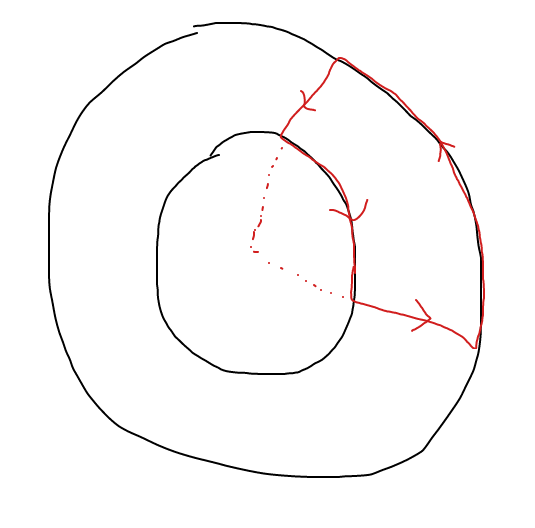
\includegraphics[width=0.45\textwidth]{curve.png}
		\caption{Sorry for the terrible sketch... The black lines are flow lines. The closed curve is given in red.}
	\end{figure}
	
	Since $\nabla \times \vec{v} = 0$, we have that the circulation is also zero:
	\begin{align*}
	\int_C \vec{v}\cdot d\vec{l} = 0.
	\end{align*}
	Since the flow lines are concentric circles, we have that 
	\begin{align*}
	\int_C \vec{v}\cdot d\vec{l} \sim  r  v_\theta \bigg\vert_{r_i}^{r_f} = 0 \implies  r v_\theta(r) = A 
	\end{align*}
	where $A$ is some constant. The angular velocity of the flow is defined via $\vec{v} = \vec{\omega} \times \vec{r}$. And since $\vec{v} = v_\theta \hat\theta$ only, $\vec{\omega} \sim (1/r^2) \hat{z}$ as desired .  
	
	
	
	\item Here we are interested only in the $z$-component of the angular momentum density $l_z = \hat z \cdot \vec{l}$. Since the flow is steady, we have $\p \vec{v}/\p t = 0$ and $\p \rho/\p t = 0$ everywhere. As a result,
	\begin{align*}
		\f{\p }{\p t} l_i = \f{\p \rho}{\p t} \epsilon_{ijk} r_j v_k +\rho \epsilon_{ijk} r_j \f{\p v_k}{\p t} = 0
	\end{align*}
	Moreover, we have
	\begin{align*}
	\vec{l} = \rho \vec{r} \times \vec{v} = \rho r \f{A}{r} \hat r \times \hat \theta = \rho A \hat z \implies l_z = \rho A
 	\end{align*}
	i.e., $l_z$ is a constant. It follows that 
	\begin{align*}
	\f{d l_z}{dt} = \f{d}{dt} \lp \hat z \cdot \vec{l} \rp = \f{\p l_z}{\p t} + (\vec{v}\cdot \nabla) l_z = 0  
	\end{align*}
	as desired since both summands are zero. Through this process, we found that the constant of proportionality is $\boxed{A = l_z/\rho}$  
	
	
	
	
\end{enumerate}



\end{document}



